\subsubsection{\texttt{RF-2}: creación de nuevos ejercicios}
\label{subsec:rf2}

Los docentes tienen la capacidad de añadir ejercicios nuevos en los cursos que imparten. En la extensión, disponen de sendos botones para añadir un solo ejercicio o varios contenidos en un mismo directorio. Para replicar este comportamiento en la aplicación web, en la pantalla que les permite visualizar el detalle de sus cursos (introducida en el \referenciaConTT{subsec:rf1}{RF-1.2}) disponen de un botón ``Add exercises'' (añadir ejercicios) que despliega un modal con todos los elementos y controles necesarios para poder crear nuevos ejercicios.

En un primer momento, el modal solicita al profesor que seleccione un directorio disponible en su sistema local de ficheros. Una vez elegido el directorio, el navegador solicitará permiso de lectura de sus contenidos a través de la \textit{File System Access API} (véase la \referenciaSeccion{subsec:tecFSA}) y, una vez concedido, se determinará automáticamente si el directorio contiene únicamente la plantilla o si tiene, además, propuesta de solución del docente. Se considera que un ejercicio dispone de plantilla de solución si su directorio raíz contiene, al menos, dos directorios \textit{template} y \textit{solution} cuyos contenidos serán tomados, respectivamente, como la plantilla y la propuesta de solución ---formato ya empleado anteriormente en la extensión---; interpretándose en otro caso que todos los contenidos conforman la plantilla. Esta exploración puede realizarse directamente en el directorio elegido o en cada subdirectorio que contenga, considerando cada uno de ellos como un nuevo ejercicio y determinando en cada caso si tienen propuesta de solución o únicamente plantilla.

\begin{figure}[ht]
    \centering
    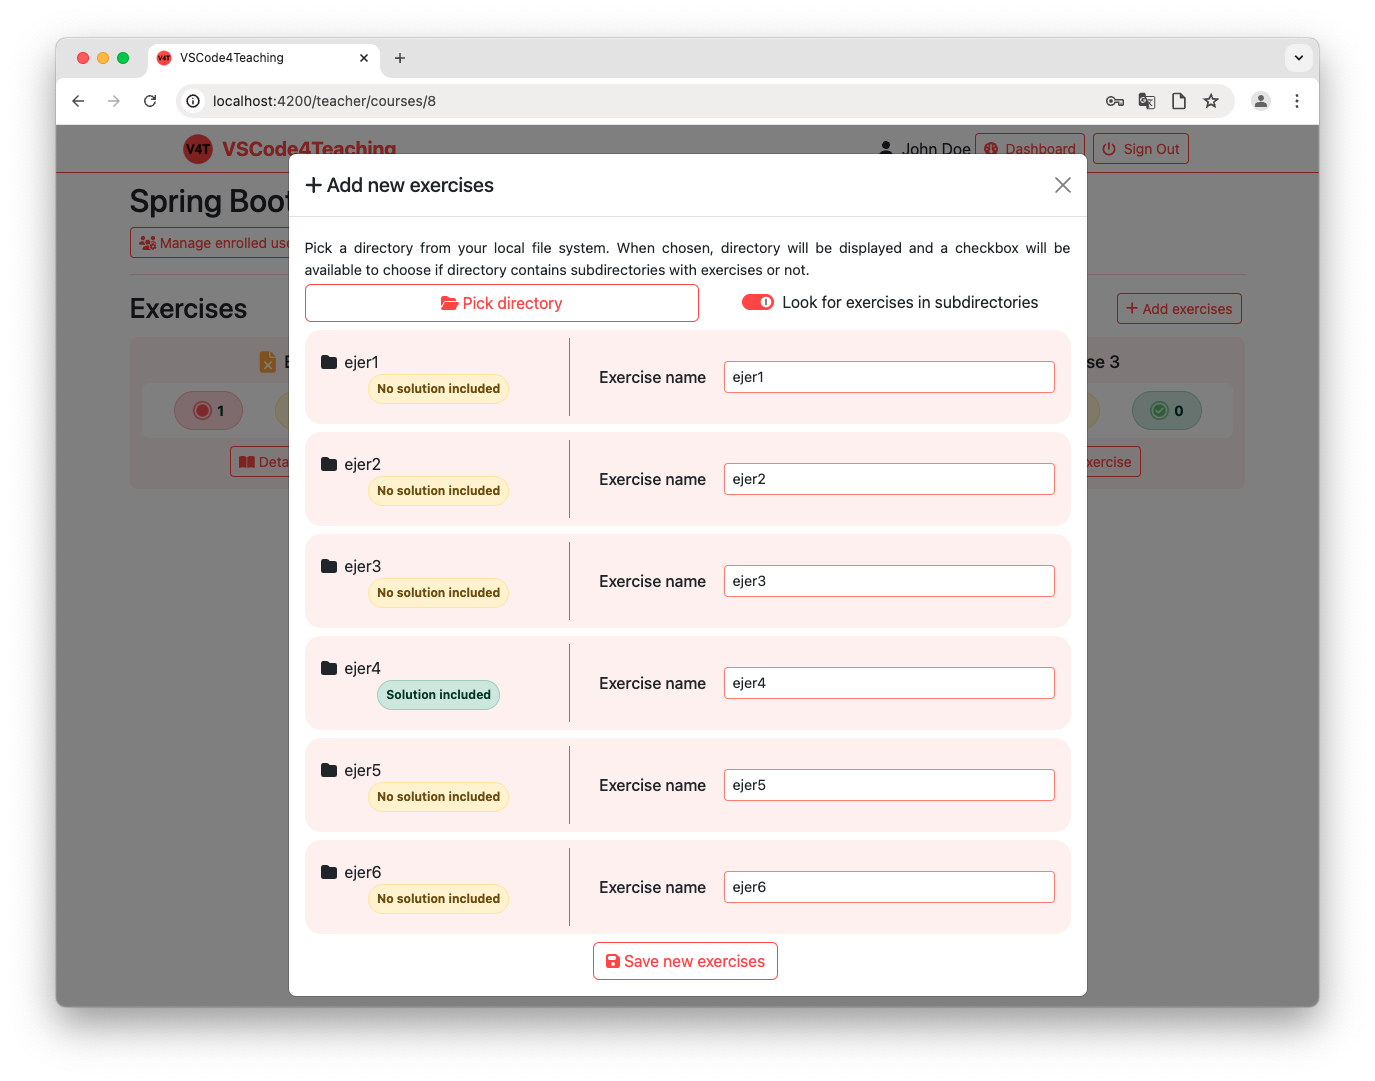
\includegraphics[width=\textwidth]{imagenes/utilizadas/4-3-implementacion/rf2-1.png}
    \caption{Ventana modal para la creación de nuevos ejercicios tras analizar los contenidos del directorio elegido.}
    \label{fig:reqf2-1}
\end{figure}

Una vez elegido un directorio y determinado si se desea emplear directamente esta carpeta o sus contenidas, se muestra una lista con los ejercicios reconocidos, mostrando para cada uno el directorio local del que proceden y un campo que permite configurar su nombre, tomando por defecto el nombre del directorio que contiene los ficheros asociados. Se muestra un ejemplo en la \referenciaFigura{fig:reqf2-1}, en la que se escoge revisar las carpetas contenidas en el directorio elegido, observando que únicamente una de ellas contiene una propuesta de resolución.

Cuando se han determinado los nombres para los ejercicios, es posible iniciar su creación. Este proceso, para cada ejercicio, ejecuta una primera petición para generar el ejercicio en el servidor y, cuando obtiene respuesta, se comprimen en el navegador los ficheros que conforman la plantilla, enviándola una vez comprimida en una nueva petición. En caso de incluir propuesta de solución, a este proceso se suma una nueva compresión y petición para guardar la propuesta de solución. Se ejecutan todos los procesos para la creación de ejercicios concurrentemente, tal como evidencia la \referenciaFigura{fig:reqf2-2}, informando a través de una barra de progreso e indicadores de estado del avance del proceso para cada ejercicio. Solo cuando hayan terminado todos los procesos, el modal podrá ser cerrado.

\begin{figure}[ht]
    \centering
    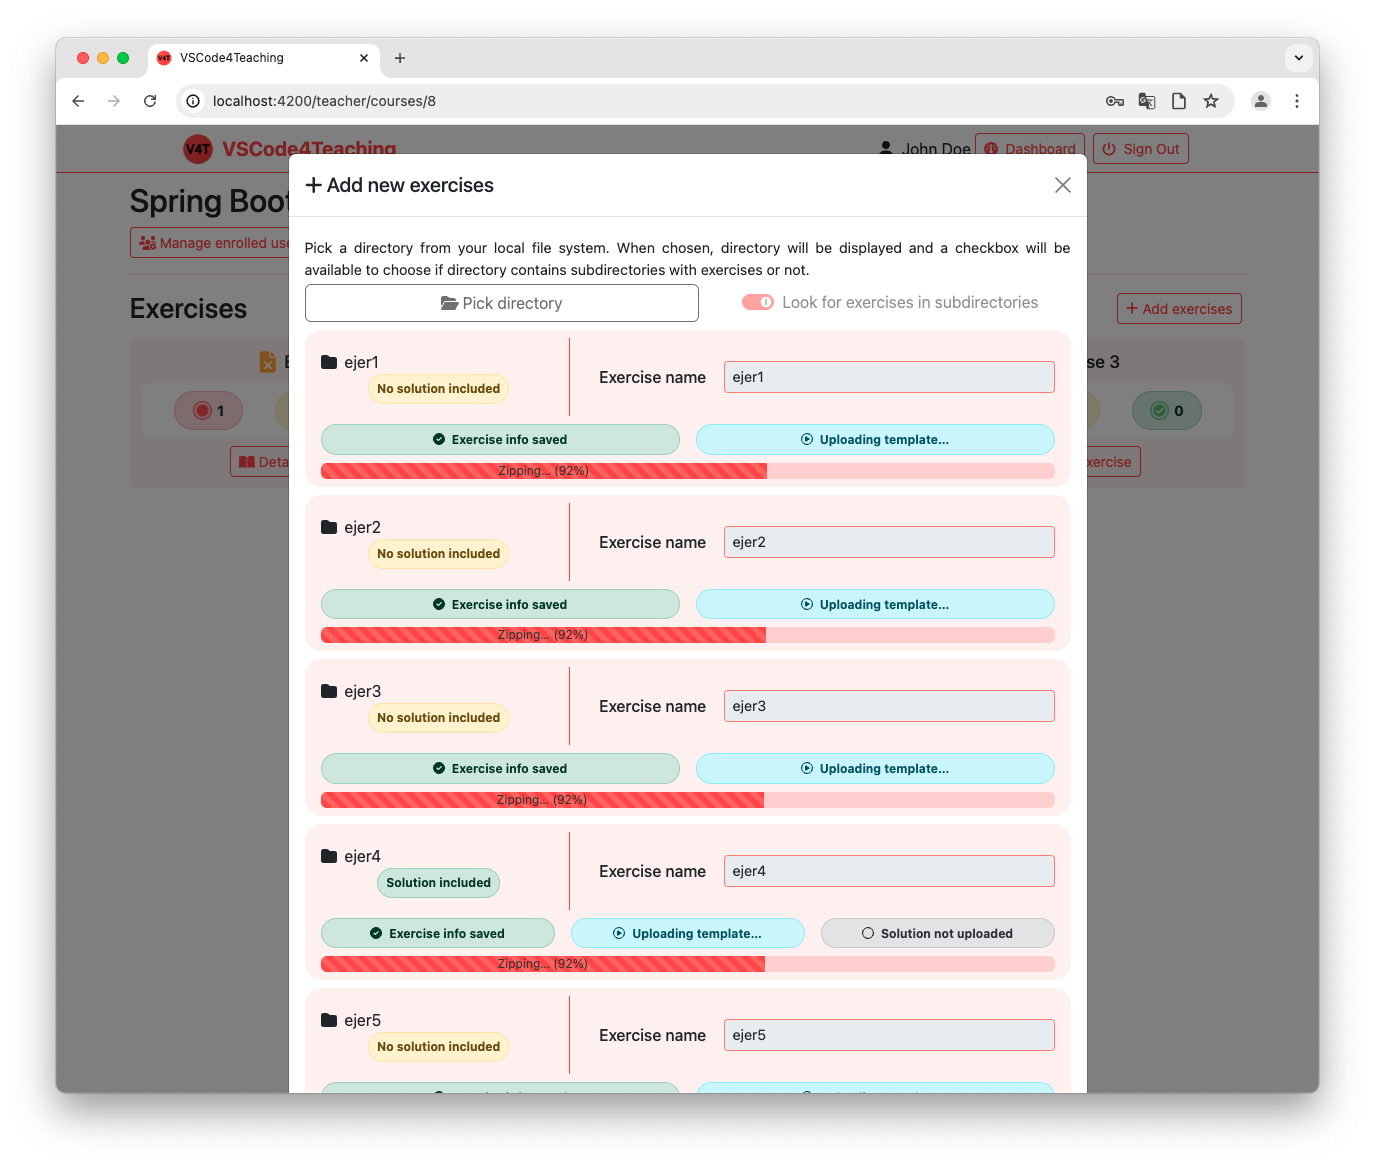
\includegraphics[width=\textwidth]{imagenes/utilizadas/4-3-implementacion/rf2-2.png}
    \caption{Instantánea de la ejecución del proceso de creación de nuevos ejercicios.}
    \label{fig:reqf2-2}
\end{figure}
